\documentclass{article}
\usepackage[utf8]{inputenc}
\usepackage{amsmath,amssymb}
\usepackage{makecell}
\usepackage[a4paper, total={6in, 9in}]{geometry}
\usepackage{authblk}
\usepackage{graphicx}
\graphicspath{{./figures/}}
\usepackage{sectsty}
\sectionfont{\fontsize{11}{15}\selectfont}
\author{Zi Han Zhao}
\affil{1001103708}
\title{CSC2125 Homework 2}
\date{}
\begin{document}
\maketitle
\renewcommand{\thesubsection}{(\alph{subsection})}
\section{Claim: account model can reduce the average size of simple transfer transactions
comparing to the UTXO model.}
The claim is true. In UTXO model, if there is a large number of UTXO inputs and outputs, 
the corresponding locking and unlocking scripts take up a large space on chain. 
In account model, however, world state is stored in the node locally. 
When being faced with the multi-account transactions, 
only the signature and the transfer value are provided for each account.\\\\
In addition, in UTXO model, each input should be verified by visiting each source of the transfer value.
The hash pointers pointing to each source also take up space on the chain.
In account model, the balance of each account is stored and no need to store hash pointers to verify.
It will save space as well.
\section{Claim: comparing to the account model in Ethereum, the UTXO model
can provide anonymous transactions if the user creates a new address for every
transaction}
The claim is true.
In UTXO model, the user is encouraged to create each new address for each transaction. 
UTXO is a stateless model. If reusing a same address, 
all of the sources of the address amount are easily visited by hash pointers.
Then the transaction history of the account address can be identified and learned.
Different addresses from one single user are created 
so that it is hard to identify the addresses belong to the same user.\\\\
In account model in Ethereum, by contrast, the user is encouraged to reuse the same account address
since each external account owns its multiple contract accounts. 
Keeping a single account is easier to manage and organize. 
It decreases the degree of privacy since all of the transactions are related with a single account.
\section{Why Ethereum introduces a GAS limit for the block? What if we remove the GAS
limit and put back the traditional block limit of 1MB like Bitcoin?}
When executing a function in smart contract, sometimes attackers can find a way to run into an infinite
loop and claim funds from another contract address. Gas limit is introduced to prevent the unlimited gas consumption.
During execution, the gas is consumed gradually by each EVM operation until reaching gas limit. 
The infinite loop execution is stopped and the function call is reverted and the account only pays for
the value of the pre-set gas limit.\\\\
If replacing gas limit with block limit, it cannot solve unlimited gas consumption during execution.
Block limit only defines the size of executed smart contract. EVM is Turing completed machine. The size of a infinite loop could be small enough in a block, which still causes the unlimited gas consumption.
\section{Ethereum sets up a different GAS amount for different EVM operations. Why?}
The computation cost of each EVM operation is different. E.g., ADD operation is cheaper than memory access operations. If the gas amount is set the same for each operation, no miners execute cost-heavy smart contract if given the same gas fee. It leads some contract transaction being never picked by miners.
\section{How to prevent reentrance attack?}
Besides limiting 2300 gas limit for code execution by using \verb|transfer()| and \verb|send()|, the smart contract designer should always change the state of the contract before transferring value. Each time of calling the function, the current state is always checked if the transfer function can be executed or not. In this way, attacker cannot re-enter the function with the same state as before and execute the transfer again.\\\\
In addition, it is always the best solution that the contract never calls another function from external contracts. External malicious contracts potentially have threats to the contract.
\section{What’s the consequence of the Integer Overflow attack in BeautyChain?}
In function \verb|batchTransfer| of BeautyChain contract, $amount = value * (\#\,of\,receivers)$ where $value$ is the input argument which the sender hopes to transfer. Then the result \verb|amount| could get overflowed to become a very small value. The outcomes are that the sender only sends a very small amount of money equal to \verb|amount|. However, each receiver get a large amount of money equal to the input \verb|value|.
\section{Other ERC20 tokens that suffered from integer
overflow vulnerabilities}
From web research, a blockchain security company called PerkShield detected that two unusual MESH and SMT token transactions. Let's look at the MESH transaction as an example:\\
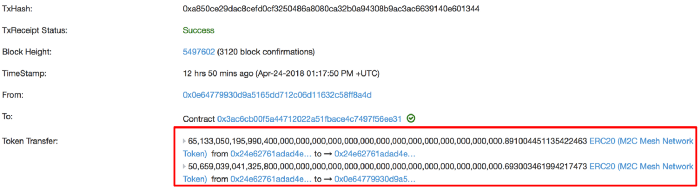
\includegraphics[width=170mm,scale=1]{mesh.png}\\
In the red circle, the address transfers a large value to himself and a large fee to another address.
The corresponding function code is:\\
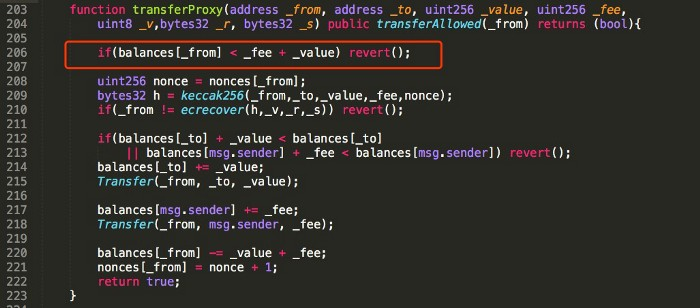
\includegraphics[width=170mm,scale=1]{meshsc.png}\\
In the red circle, the addition between fee and value is over $2^{256}-1$, which becomes a very small value.
It never calls \verb|revert()|. 
Therefore, after passing \verb|revert()|, line 215 will transfer to himself with a large value \verb|_value| but the balance of himself 
\verb|balances[_from]|
doesn't own such a large value.
\section{What kind of the failure causes the MakerDAO event? Is it a contract design
failure or a bug? What could do to strengthen such Defi protocols?}
The main reason is network congestion. 
First, price oracle cannot update price in time. 
When the price is updated, the vaults are suddenly liquidated as unexpected. 
Still due to network congestion, a keeper successfully wins the auction by 0 Dai without no other bidders. 
The cause of network congestion is that a large number of transactions occurs since ETH price dropped significantly.\\\\
It is a design failure because there is no problem for MakerDAO contracts itself,
but under the ETH floating price environment, 
it is unexpected for testers to build the contract design under such a congested network.\\\\
In terms of enhancement of such DeFi protocols, try to reduce the dependency about the volatile currency
since it is unexpected and untestable to build and run the protocol in practical currency environment.
Also, price oracle plays a key rule of price updating. The designer should reduce the delay of price update under network congestion. In addition, network congestion is a big issue in the problem. The protocol designer should test the design feasibility under much lagged network.
\section{Why Flash loan can be borrowed without any collateral? Why Flash loan is
primarily used by hackers for launching attacks on DeFi protocols?}
Here are three steps:
1)The loan lending, 2)trading with loan in DeFi 
and 3)the loan repaying. They are executed in one transaction in a contract.
Before repaying, the loan receiver can do everything with loan. 
If no repaying on time, the transaction execution will throw an execution error and be reverted to the original account state,
i.e., no loan lending occurs ever. Therefore, there is no need to put collaterals for loan.\\\\
By flash loan, attackers don't need any assets and collaterals and steal a much large amount of
cryptocurrency loan without any investment in a short time. 
Any effective mallicious manipulation of market needs a large amount of assets 
and flash loan gives the chance. 
Also, since the price oracles of each DeFi protocol fail under the big changes of each currency, the large amount which is easily borrowed by flash loan hits the currency market more efficiently.
\end{document}